\newcommand\note[2]{\textbf{#1: }\emph{#2}}
\newcommand\answer[1]{\note{Answer}{#1}}
\newcommand\grading[1]{\note{Grading}{#1}}
\newcommand\responses[1]{\note{Responses}{#1}}

\chapter{User study materials}
\label{appendix:userstudy}

This appendix includes various materials used in the Raft user study
(Chapter~\ref{userstudy}):
\begin{compactitem}
\item Section~\ref{appendix:userstudy:raftquiz} contains the Raft quiz
questions, answers, and grading rubric.
\item Section~\ref{appendix:userstudy:paxosquiz} contains the Paxos quiz
questions, answers, and grading rubric.
\item Section~\ref{appendix:userstudy:survey} contains the survey
and the open-ended comments and feedback received from the participants.
\item Section~\ref{appendix:userstudy:supporting} contains the summaries of
the Raft and Paxos algorithms made available to participants during the study.
\end{compactitem}

\section{Raft quiz}
\label{appendix:userstudy:raftquiz}

\note{Grading note}{Where points are taken away for incorrect
information, every section of every question still has a minimum of 0
points.}

\begin{enumerate}
\item[1.] (4 points)
Each figure below shows a possible log configuration for a Raft server
(the contents of log entries are not shown; just their indexes and
terms). Considering each log in isolation, could that log configuration
occur in a proper implementation of Raft? If the answer is ``no,''
explain why not.

\begin{enumerate}[(a)]
\item \ \\ 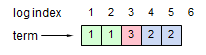
\includegraphics[scale=0.75]{userstudymaterials/legala}

\answer{No: terms increase monotonically in a log.
\\
Specifically, the leader that created entry (4,2) could only have
received (3,3) from a leader with current term $\geq$ 3, so its current term
would also be $\geq$ 3. Then it could not create (4,2).
}

\item \ \\ 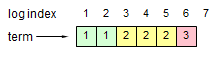
\includegraphics[scale=0.75]{userstudymaterials/legalb}

\answer{Yes
}

\item \ \\ 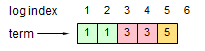
\includegraphics[scale=0.75]{userstudymaterials/legalc}

\answer{Yes
}

\item \ \\ 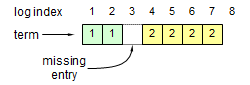
\includegraphics[scale=0.75]{userstudymaterials/legald}

\answer{No: logs cannot have holes.
\\
Specifically, leaders only append to their logs, and the consistency
check in AppendEntries never matches a hole.
}
\end{enumerate}

\grading{4 points total
\\
One point per part.
\\
If the answer is yes, saying ``yes'' earns 1 point. Saying ``no'' earns
no points. Any supporting explanations are ignored.
\\
If the answer is no, saying ``no'' earns half of the point, and a
correct explanation earns the other half. Not much supporting
explanation is required. Saying ``yes'' earns no points, and any
accompanying explanation is ignored.
}

\item[2.] (6 points)
The figure below shows the state of the logs in a cluster of 5 servers
(the contents of the entries are not shown). Which log entries may
safely be applied to state machines? Explain your answer.

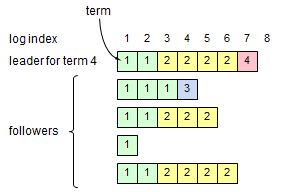
\includegraphics[scale=0.75]{userstudymaterials/committed}

\answer{Entries (1,1) and (2,1) may be safely applied:
\\
If an entry is not stored on a quorum, it cannot be applied safely.
This is because this minority can fail, and the other servers (which
form a majority) can proceed with no knowledge of the entry.
\\
Thus, we need only consider entries (1,1), (2,1), (3,2), (4,2), (5,2).
\\
We need to figure out which ones could be elected leader, and see if
they could cause these entries to be removed.
\\
Server 2 can be elected leader because its log is at least as
complete as S3, S4, and S5. It could then cause servers to remove
entries (3,2), (4,2), and (5,2), so those entries are not safe to apply.
\\
So now we're left with entries (1,1), (2,1) as possibly safe to apply.
\\
Servers 3 and 4 can't be elected leader because their logs are not
complete enough. Server 5 can be elected leader, but it contains (1,1)
and (2,1).
\\
Therefore, only entries (1,1) and (2,1) are safe to apply.
}

\grading{
6 points total
\\
3 points for saying ``entries (1,1) and (2,1)'' or ``entries 1 and 2''
(since there is no ambiguity). No partial credit is awarded for these 3
points, but responses with an incorrect answer may still be awarded
partial credit for the explanation.
\\
3 points for the explanation:
\\
+ 1 point for saying the entry must be stored on a quorum
\\
+ 2 points for saying that server 2 may be elected leader, which threatens
entries past index 2.
\\
An answer that says ``1 and 2 because entries from term 2 can't be
committed until one of the entries from the leader's term reaches a
majority of servers'' receives 4.5 points (we got 3 answers like this;
it's correct but not clear whether the participants understood why).
\\
The incorrect answer of ``entries 1--5 because they are stored on a
majority'' gets 1 point.
\\
The incorrect answer of ``entries 1--6 because
they are stored on a majority'' gets 0 points (entry 6 is not).
}

\item[3.] (10 points)
Consider the figure below, which displays the logs in a cluster of 6
servers just after a new leader has just been elected for term 7 (the
contents of log entries are not shown; just their indexes and terms).
For each of the followers in the figure, could the given log
configuration occur in a properly functioning Raft system? If yes,
describe how this could happen; if no, explain why it could not happen.

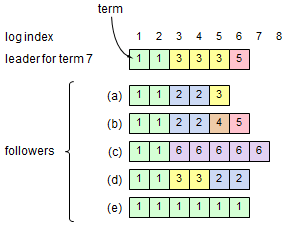
\includegraphics[scale=0.75]{userstudymaterials/inconsistency}

\answer{
\begin{compactenum}
\item[a)]
No. Entry (5,3) uniquely identifies a log prefix (by the
AppendEntries consistency check), but this follower has entry (5,3) and
a different log prefix before it than the leader.
\item[b)]
No. Entry (6,5) uniquely identifies a log prefix (by the
AppendEntries consistency check), but this follower has entry (6,5) and
a different log prefix before it than the leader.
\item[c)]
Yes. Since we can't say much about the other servers in the cluster,
this server could have been leader in term 6 with a starting log of
(1,1), (2,1) and could have written a bunch of entries to its log and
not communicated with our current leader of term 7. This assumes that
entries (3,3), (4,3), (5,3), and (6,5) were not committed in term 5,
which is possible.
\item[d)]
No. Terms increase monotonically in a log.
Specifically, the leader that created entry (5,2)
could only have received (4,3) from a leader with current term $\geq$ 3, so
its current term would also be $\geq$ 3. Then it could not create (5,2).
\item[e)]
Yes. For example, (e) is the leader for term 1 and commits entries
(1,1) and (2,1), then becomes partitioned from the other servers but
continues processing client requests.
\end{compactenum}
}

\grading{
10 points total
\\
Two points per part:
\\
+ 1 for the boolean,
\\
+ 1 for a correct explanation.
\\
If the boolean is incorrect, no points are awarded for the explanation.
\\
If the boolean is correct, not much supporting explanation is required.
}

\item[4.] (5 points)
Suppose that a hardware or software error corrupts the nextIndex value
stored by the leader for a particular follower. Could this compromise
the safety of the system?  Explain your answer briefly.

\answer{No.
\\
If the nextIndex value is too small, the leader will send extra
AppendEntries requests. Each will have no effect on the follower's log
(they will pass the consistency check but not conflict with any entries
in the follower's log or provide any entries to the follower that the
follower didn't already have), and the successful response will indicate
to the leader that it should increase its nextIndex.
\\
If the nextIndex value is too large, the leader will also send extra
AppendEntries requests. The consistency check will fail on these,
causing the follower to reject the request and the leader to decrement
nextIndex and retry.
\\
Either way, this is safe behavior, as no critical state is modified in
either case.
}

\grading{
5 points total
\\
+ 1 point for saying ``no''.
\\
+ 2 points for explaining what happens if nextIndex is too small. 
\\
+ 2 points for explaining what happens if nextIndex is too large.
\\
Answers that say a follower would truncate its log when nextIndex is too
small receive -1 points, as that could result in a safety violation.
\\
If the boolean is incorrect, partial credit may still be awarded for
correct explanations.
}


\item[5.] (5 points)
Suppose that you implemented Raft and deployed it with all servers in
the same datacenter. Now suppose that you were going to deploy the
system with each server in a different datacenter, spread over the
world. What changes would you need to make, if any, in the wide-area
version of Raft compared to the single-datacenter version, and why?

\answer{We'd need to set the election timeouts higher: the expected
broadcast time is higher, and the election timeout should be much higher
than the broadcast time so that candidates have a chance to complete an
election before timing out again. The rest of the algorithm does not
require any changes, since it does not depend on timing.
}

\grading{
5 points total
\\
For full credit, an answer needs to include increasing the election timeout
and as justification mention increased latency or some sort of livelock.
\\
Answers that talk about ``increasing timeouts'' without specifically
mentioning elections receive up to 3.5 points (this affects 4 answers).
\\
Unnecessary or optional changes (performance improvements) are ignored
if correctly identified as such.
\\
Negative points are awarded for other changes identified as
required.
}

\item[6.] (10 points)
Each follower stores 3 pieces of information on its disk: its current
term, its most recent vote, and all of the log entries it has accepted.

\begin{enumerate}[(a)]
\item Suppose that the follower crashes, and when it restarts, its most
recent vote has been lost. Is it safe for the follower to rejoin the
cluster (assuming no modifications to the algorithm)? Explain your
answer.

\answer{%
No. This would allow a server to vote twice in the same term, which
would then allow multiple leaders per term, which breaks just about
everything.
\\
For example, with 3 servers:
\\
S1 acquires S1 and S2's votes and becomes leader of term 2.
\\
S2 restarts and forgets it voted in term 2.
\\
S3 acquires S2 and S3's votes and becomes the second leader of term 2.
\\
Now S1 and S3 can commit distinct entries in term 2 with the same index and terms but different values.
}

\item Now suppose that the follower's log is truncated during a crash,
losing some of the entries at the end. Is it safe for the follower to
rejoin the cluster (assuming no modifications to the algorithm)? Explain
your answer.

\answer{%
No. This would allow a committed entry to not be stored on a quorum,
which would then allow some other entry to be committed for the same
index.
\\
For example, with 3 servers.
\\
S1 becomes leader in term 2 and appends index=1, term=2, value=X on itself and S2.
\\
S1 sets its committedIndex to 1 and returns to the client that X is committed.
\\
S2 restarts and loses the entry from its log.
\\
S3 (with an empty log) becomes leader in term 3, since its empty log is at least as complete as S2's.
\\
S3 appends index=1, term=3, value=Y on itself and S2.
\\
S3 sets its committedIndex to 1 and returns to the client that Y is committed.
}

\end{enumerate}

\grading{
10 points total
\\
5 points per part:
\\
+ 1 point for the boolean,
\\
+ 4 points for a correct explanation (the detailed scenarios above are not
required)
\\
For full credit on part (a), answers needed to include that this would
allow multiple leaders to be elected for the same term, not just that a
follower could vote twice.
\\
If the boolean is incorrect, no points are awarded for the explanation.
}

\item[7.] (10 points)
As described in the video, it's possible for a leader to continue
operating even after other servers have decided that it crashed and
elected a new leader. The new leader will have contacted a majority of
the cluster and updated their terms, so the old leader will step down as
soon as it communicates with any of these servers. However, in the
meantime it can continue to act as leader and issue requests to
followers that have not yet been contacted by the new leader;
furthermore, clients may continue to send requests to the old leader. We
know that the old leader cannot commit any \emph{new} log entries it
receives after the election has completed, since it would need to
contact at least one of the servers in the electing majority to do this.
But, is it possible for an old leader to execute a successful
AppendEntries RPC that completes the commitment of an old log entry that
was received before the election started? If so, explain how this could
happen, and discuss whether or not this will cause problems for the Raft
protocol. If this cannot happen, explain why.

\answer{%
Yes. This can only happen if the new leader also contains the entry
being committed, so it will not cause problems.
\\
Here's an example of this happening with 5 servers:
\\
S1 with an empty log becomes leader for term 2 with votes S1, S2, and
S3.
\\
S1 completes appending index=1, term=2, value=X to itself and S2.
\\
S2 with index=1, term=2, value=X in its log becomes leader for term 3
with votes S2, S4, S5.
\\
S1 completes appending index=1, term=2, value=X to S3.
\\
At this point, S1 has completed commitment of index=1, term=2, value=X,
even though it is no longer the current leader.
\\
\\
This behavior is safe because any new leader must also contain the
entry, and so it will persist forever:
\\
The entry must be stored on some server S that votes for the new leader
L, and it must be stored on S \emph{before} S votes for that new leader.
The log completeness check says that S may only vote for L if:
\\
 L.lastLogTerm $>$ S.lastLogTerm or
\\
 (L.lastLogTerm == S.lastLogTerm and L.lastLogIndex $\geq$ S.lastLogIndex)
\\
If L is the first leader after S, we must be in the second case, and
then L must contain every entry that S has, including the one we're
worried about.
\\
If L' is the second leader after S, L' could only have a larger last
term than S if it received entries from L. But L must have replicated
the entry we're worried about to L' prior to replicating any of its own
entries to L', so this is also safe.
\\
And this argument holds inductively for all future leaders.
}

\grading{
10 points total
\\
4 points for showing this is possible:
\\
+ 1 point for saying ``Yes, it is possible''
\\
+ For the remaining 3 points, answers must include that the deposed
leader completed an AppendEntries request to one of the voters of the
new leader before that server voted.
\\
6 points for arguing that it is not a problem:
\\
+ 1 point for saying ``It's not a problem.''
\\
+ For the remaining 5 points, answers must include that because some
voter must have the entry, the log completeness check guarantees that
the new leader must also have the entry.
\\
No points awarded for saying this cannot happen.
\\
Credit for the scenario may be awarded even if the answer argues that
this is a problem for Raft.
}

\item[8.] (10 points)
During configuration changes, if the current leader is not in \cnew{},
it steps down once the log entry for \cnew{} is committed. However, this
means that there is a period of time when the leader is not part of the
cluster it's leading (the current configuration entry stored on the
leader is \cnew{}, which does not include the leader). Suppose the
protocol were modified so that the leader steps down as soon as it
stores \cnew{} in its log, if \cnew{} doesn't include the leader. What's
the worst that could happen with this approach?

\answer{%
Depending on the interpretation of the algorithm, there are two possible
correct answers.
\\
Answer 1 assumes an implementation wherein once a server is not
part of its current configuration, it does not become candidate anymore.
The problem is that another server in \cold{} could then be
elected as leader, append \cnew{} to its log, and immediately
step down.
\\
Worse yet, this could repeat for a majority of the servers in \cold{}. It
couldn't repeat more than that because once a majority of \cold{} stores
the \cnew{} entry, no server from \cold{} without this entry could be
elected due to the log completeness check (a majority of \cold{},
required for \cboth{}, would no longer grant its vote to this server).
\\
After this, a server in \cnew{} would have to get elected, and
the cluster would continue. So the worst case is really just running
through up to about $|$\cold{}$|$/2 extra elections and election
timeouts.
\\
Answer 2 assumes a na\"ive implementation that allows a server that is not
part of its current configuration to still become candidate. In this
case, the worst thing that could happen is that the leader gets elected
again as soon as it steps down (its log is still complete), then steps
down again, then repeats infinitely.
}

\grading{
10 points total
\\
For full credit, an answer needs to identify that a server not in
\cnew{} can be elected, that this can repeat, include a reasonable bound
on this repetition, and mention that this causes an availability or
liveness problem.
}

\end{enumerate}

\section{Paxos quiz}
\label{appendix:userstudy:paxosquiz}

\note{Grading note}{Where points are taken away for incorrect
information, every section of every question still has a minimum of 0
points.}


\begin{enumerate}
\item[1.] (4 points)
Each figure below shows a possible log configuration for a Multi-Paxos
server (the number in each log entry gives its acceptedProposal value).
Considering each log in isolation, could that log configuration occur in
a proper implementation of Multi-Paxos?

\vspace{3ex}
\begin{compactenum}
\item[a)]
\ \\ 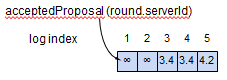
\includegraphics[scale=0.75]{userstudymaterials/paxosLoga}
\\ Yes or No?
\\ \answer{Yes}
\item[b)]
\ \\ 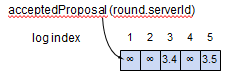
\includegraphics[scale=0.75]{userstudymaterials/paxosLogb}
\\ Yes or No?
\\ \answer{Yes}
\item[c)]
\ \\ 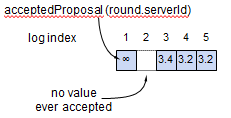
\includegraphics[scale=0.75]{userstudymaterials/paxosLogc}
\\ Yes or No?
\\ \answer{Yes}
\item[d)]
\ \\ 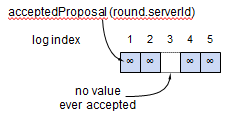
\includegraphics[scale=0.75]{userstudymaterials/paxosLogd}
\\ Yes or No?
\\ \answer{Yes}
\end{compactenum}

\grading{
1 point per boolean (no partial credit)
}

\item[2.] (6 points)
In Basic Paxos, suppose that a cluster contains 5 servers and 3 of them
have accepted proposal 5.1 with value X. Once this has happened, is it
possible that any server in the cluster could accept a different value
Y? Explain your answer.

\answer{%
Yes. If it's S1, S2, and S3 that have accepted (5.1, X), other servers
could still accept Y if it has a stale proposal number.
\\
For example, S4 could prepare 3.4 and discover no values. Then S1 could
prepare 5.1 on just S1, S2, S3. Then S1 could complete accepts on just
S1, S2, S3. And S4 can still complete accepts on S4 and S5 with
(3.4, Y).
}

\grading{
6 points total
\\
2 points for saying ``Yes'', and 4 points for the accompanying
explanation. The explanation must indicate that Y's proposal is
concurrent with or numbered less than 5.1 (otherwise, $-2$ points).
\\
The incorrect answer ``No, because any new proposal must discover (5.1,
X) in its prepare phase'' receives 2 points.
\\
Other incorrect answers with ``No'' receive no credit.
}

\item[3.] (10 points)
Suppose that a server has just decided to act as leader in Multi-Paxos,
and that no other servers are currently acting as leaders. Furthermore,
assume that the server continues as leader for a period of time,
arranging for many commands to be chosen for log entries, and that no
other server attempts to act as leader during this period.

\begin{compactenum}
\item[a)]
What is the lower bound on the number of rounds of Prepare RPCs that the
server must issue during this period? Explain your answer, and be as
precise as possible.

\answer{%
The lower bound is 1 round of Prepare RPCs, if a quorum of Prepare
responses are returned right away that have noMoreAccepted=true.
}
\item[b)]
What is the upper bound on the number of rounds of Prepare RPCs that the
server must issue during this period? Explain your answer, and be as
precise as possible.

\answer{%
The upper bound is one round of Prepare RPCs for each slot that is not
chosen on the leader for which any acceptor has accepted any proposal.
This can happen if every time the leader issues a prepare for one of its
unchosen slots, it discovers an acceptor that has already accepted some
value; then it needs to adopt this value for this slot and continue
trying with the next slot.
}
\end{compactenum}

\grading{
10 points total
\\
5 points per part
\\
For part a:
\\
+ 2 points for saying ``1''
\\
+ 3 points for the accompanying explanation
\\
The explanation must include some mention of noMoreAccepted or the
concept behind it.
\\
For part b:
\\
+ 3 points for saying the number of entries a follower has accepted
\\
+ 2 points for subtracting out the ones that are chosen on the leader
\\
An answer which is lacking precision that says ``the upper bound is
arbitrarily large'' but which has a correct explanation as to why more
than 1 is necessary receives 2 points.
\\
Answers that just say ``until noMoreAccepted is true for a majority''
receive 2 points (true, but they could have gotten this off the slide
without understanding).
\\
Answers that are O(1) or O(Len(leader's log)) for part (b) are awarded
no credit.
}

\item[4.] (5 points)
When an acceptor is marking entries accepted using the
firstUnchosenIndex provided by the proposer, it must first check the
proposal number in the entries that it marks. Suppose it skipped this
check: describe a scenario where the system would misbehave.

\note{Errata}{The question should have read ``marking entries chosen''
instead of ``marking entries accepted''. The quizzes used in our study
contained the error, which we did not notice until grading the
responses.}

\answer{The misbehavior that can arise is a server marking a value as
chosen when a different value has been chosen. This requires a minimum
of 2 competing proposals, 3 servers, and 2 log entries to show:
\\
S1 completes a round of prepare for n=1.1, index=1 with S1, S2.
\\
S1 completes only one accept for n=1.1, v=X, index=1 with S1 (itself).
\\
S2 completes a round of prepare for n=2.2, index=1 with S2, S3 and gets
back noMoreAccepted=true from both.
\\
S2 completes a round of accept for n=2.2, v=Y, index=1 with S2, S3.
\\
S2 marks index 1 as chosen.
\\
S2 completes a round of accept for n=2.2, v=Z, index=2,
firstUnchosenIndex=2 with S1, S2, and S3.
\\
Here, S1 would have misbehaved by setting n=1.1, v=X as chosen and
applying X to its state machine. This is incorrect, since in fact Y was
chosen.
}

\grading{
5 points total
\\
Unfortunately, most of the answers were not as specific as we would have
liked for the scenario.
\\
Full credit required identifying that the previously accepted
\emph{value} was different from the chosen value on the proposer, and
not just that the proposal number was different. This helps separate
people that regurgitated the material from people that had some
understanding of why the algorithm is the way it is. Answers missing
this component received up to 4 points (typically 2--3), depending on how
well they showed understanding.
\\
Since we messed up the wording in the question, no points were taken off
on this question for confusing the words ``accepted'' and ``chosen'' in
the answer (answers were read with these words exchanged in any way
possible to give the answer the maximum number of points).
}

\item[5.] (5 points)
Suppose that the two parts of a proposal number (round number and unique
server id) were exchanged, so that the server id is in the high-order
bits.

\begin{compactenum}
\item[a)]
Would this compromise the safety of Paxos? Explain your answer briefly.

\answer{No, since safety only requires proposals to be uniquely numbered
(for a given index in Multi-Paxos). Because server IDs are unique to
each server and round numbers still monotonically increase, this
uniqueness is preserved.
}
\item[b)]
Would this compromise the liveness of Paxos? Explain your answer briefly.

\answer{Yes, for example, the server with the largest ID could issue a
Prepare RPC to every server in the cluster and then permanently fail. No
other proposer would then be able to make any progress, since the
remaining servers' minProposal values would be too high for the
remaining proposers.
}
\end{compactenum}

\grading{
5 points total
\\
+ 2 points for safety
\\
+ 3 points for liveness
\\
For safety, saying ``no'' is worth 1 point, and a correct explanation is
worth 1 point. Not much supporting explanation is required. Saying
``yes'' earns no points, and any accompanying explanation is
ignored.
\\
For liveness, saying ``yes'' is worth 1 point, and a correct explanation
is worth 2 points. Saying ``no'' earns no points, and any
accompanying explanation is ignored.
}

\item[6.] (10 points)
Suppose that a proposer executes the Basic Paxos protocol with an initial value
of v1, but that it crashes at some (unknown) point during or after the
execution of the protocol. Suppose that the proposer restarts and reexecutes
the protocol from the beginning with the same proposal number used previously,
but with a different initial value of v2. Is this safe? Explain your answer.

\answer{%
No. Different proposals must have distinct proposal numbers. Here's an
example of something bad that can happen using 3 servers:
\\
S1 completes Prepare(n=1.1) with S1, S2.
\\
S1 completes Accept(n=1.1, v=v1) with S1.
\\
S1 restarts.
\\
S1 completes Prepare(n=1.1) with S2, S3 (and discovers no accepted proposals).
\\
S1 completes Accept(n=1.1, v=v2) with S2, S3.
\\
S1 responds to the client that v2 has been chosen.
\\
S2 completes Prepare(n=2.2) with S1, S2 and gets back:
\\
 from S1: acceptedProposal=1.1, acceptedValue=v1,
\\
 from S2: acceptedProposal=1.1, acceptedValue=v2,
\\
S2 chooses to use v1 arbitrarily.
\\
S2 completes Accept(n=2.2, v=v1) with S1, S2, S3.
\\
S2 responds to some client that v1 was chosen.
\\
\\
A different problem that can occur involves a request from before the crash being delivered after the crash:
\\
S1 completes Prepare(n=1.1) with S1, S2.
\\
S1 completes Accept(n=1.1, v=v1) with S1.
\\
S1 sends Accept(n=1.1, v=v1) to S2 and S3, but they don't receive it yet.
\\
S1 restarts.
\\
S1 completes Prepare(n=1.1) with S2, S3 (and discovers no accepted proposals).
\\
S1 completes Accept(n=1.1, v=v2) with S2, S3.
\\
S1 responds to the client that v2 has been chosen.
\\
Now S2 and S3 receive the Accept(n=1.1, v=v1) request and overwrite their acceptedValue to be v1.
\\
The state of the cluster is now that v1 is chosen, even though a client has been told that v2 was chosen.
}

\grading{
10 points total
\\
2 points for saying ``no'', and 8 points for a correct explanation
\\
For full credit, answers needed to explain that v2's prepare phase did
not discover v1 and include some violation of safety.
\\
Saying ``yes'' earns no points, and any accompanying explanation is
ignored.
}

\item[7.] (10 points)
In a successful Accept RPC the acceptor sets its minProposal to n (the proposal
number in the Accept RPC). Describe a scenario where this actually changes the
value of minProposal (i.e., minProposal isn't already equal to n). Describe a
scenario where the system would behave incorrectly without this code.

\answer{%
Working backwards, we need a server to receive an Accept that did not
receive a Prepare, since otherwise its minProposal would be up to date.
And for this to matter, a subsequent Accept needs to incorrectly not be
rejected.
\\
Using Basic Paxos and 5 servers.
\\
S1 completes Prepare(n=1.1) with S1, S2, S3 (and discovers no accepted proposals).
\\
S5 completes Prepare(n=2.5) with S3, S4, S5 (and discovers no accepted proposals).
\\
S5 completes Accept(n=2.5, v=X) with S2, S3, S5. This is where S2's minProposal would be to 2.5 upon processing the Accept request.
\\
S5 returns to the client that X is chosen.
\\
S1 completes Accept(n=1.1, v=Y) with S2. This would normally be rejected, but would be accepted if S2's minProposal was not updated during Accept.
\\
S3 completes Prepare(n=3.3) with S1, S2, S4 (and discovers n=1.1, v=Y).
\\
S3 completes Accept(n=3.3, v=Y) with S1, S2, S3, S4, S5.
\\
S3 returns to a client that Y is chosen.
}

\grading{
10 points total
\\
+ 4 points for the first three steps showing how minProposal can be set
during Accept.
\\
+ 6 points for showing how the system misbehaves. For full credit, this
must include a safety violation.
}


\item[8.] (10 points)
Consider a configuration change in Multi-Paxos, where the old configuration
consists of servers 1, 2, and 3, and the new configuration consists of servers
3, 4, and 5.  Suppose that the new configuration has been chosen for entry N in
the log, and entries N through N+$\alpha$ (inclusive) have also been chosen.
Suppose that at this point the old servers 1 and 2 are shut down because they
are not part of the new configuration. Describe a problem that this could cause
in the system.

\answer{%
This could cause a liveness problem for the new cluster because
firstUnchosenIndex on those servers may be less than N+$\alpha$.
\\
For example in the worst case, server 3 might have failed permanently,
and servers 1 and 2 would have made no attempt to transfer any values to
servers 4 and 5 (using just the algorithm presented in the lecture).
Then, try as they might, servers 4 and 5 will never be able to learn the
chosen values for slots 1 through N+$\alpha$-1 (inclusive), since they
can't communicate with servers 1, 2, or 3. Server 4 and 5's state
machines would never be able to advance beyond their initial
state.
}

\grading{
10 points total
\\
A complete answer must say that the new servers are missing chosen
entries and dismiss server 3 as the solution.
\\
Answers received up to 7 points if they implied server 3 must have all
information (it can fail). Answers received up to 8 points if they
implied server 3 having all information is sufficient (it can fail).
\\
No points are awarded for incorrectly saying there is no problem.
\\
No points are awarded for incorrectly saying that some slots in the
range $1$ through $N - 1$ (inclusive) may not have been chosen. That's
because $N$ through $N+\alpha$ (inclusive) chosen implies 
$1$ through $N+\alpha$ (inclusive) are chosen by the definition
of $\alpha$.
}

\end{enumerate}

\section{Survey}
\label{appendix:userstudy:survey}

\begin{enumerate}
\item Please rate any prior exposure you've had to Paxos.

\begin{compactitem}
\item I had never seen it before
\item I had seen it before but didn't remember it
\item I had seen it before but remembered only a little bit
\item I had seen it before and remembered quite a bit
\item I had seen it before and consider myself an expert
\end{compactitem}

\responses{Responses are presented in Figure~\ref{fig:userstudy:surveypaxos}.}

\item Please rate any prior exposure you've had to Raft.

\begin{compactitem}
\item I had never seen it before
\item I had seen it before but didn't remember it
\item I had seen it before but remembered only a little bit
\item I had seen it before and remembered quite a bit
\item I had seen it before and consider myself an expert
\end{compactitem}

\responses{No participants reported having seen Raft before.}

\item Do you think the video lectures were roughly equal in quality, given the nature of the material being presented?

\begin{compactitem}
\item Paxos lecture was much better
\item Paxos lecture was somewhat better
\item They were roughly equal
\item Raft lecture was somewhat better
\item Raft lecture was much better
\end{compactitem}

\responses{Responses are presented in Figure~\ref{fig:userstudy:surveyfair}.}

\item Do you think the quizzes were roughly equal in terms of testing your understanding of the material?

\begin{compactitem}
\item Paxos questions were unfairly hard
\item Paxos questions were somewhat harder
\item They were roughly equal
\item Raft questions were somewhat harder
\item Raft questions were unfairly hard
\end{compactitem}

\responses{Responses are presented in Figure~\ref{fig:userstudy:surveyfair}.}

\item Suppose you were working at a company and it is your job to implement a
replicated state machine. Which algorithm would be easier to implement in a
functioning, correct, and efficient system?

\begin{compactitem}
\item Paxos would be much easier
\item Paxos would be somewhat easier
\item They would be roughly equal
\item Raft would be somewhat easier
\item Raft would be much easier
\end{compactitem}

\responses{Responses are presented in Figure~\ref{fig:userstudy:survey}.}

\item Suppose you had to explain either Raft or Paxos to a CS graduate student who
hadn't seen either one previously. Which would be easier to explain?

\begin{compactitem}
\item Paxos would be much easier
\item Paxos would be somewhat easier
\item They would be roughly equal
\item Raft would be somewhat easier
\item Raft would be much easier
\end{compactitem}

\responses{Responses are presented in Figure~\ref{fig:userstudy:survey}.}

\item Do you have any additional comments?

\responses{
The participants' responses are reproduced below in random order,
exactly as submitted (errors included):
}
\begin{itemize}
\item \emph{I was forced to go back and re-watch parts of the Paxos lecture in order to answer the quiz questions. I could answer most of the Raft questions from memory.}
\item \emph{I started a bit late on watching the videos.  Without as much time to fully absorb the material before taking the quizzes, I left a couple of parts incomplete. \\ I liked the one-slide summary near the beginning of the Raft lecture.}
\item \emph{Both are super complex!}
\item \emph{Good job on the lecture videos.}
\item \emph{Raft might be simpler, but the lecture on it was much harder to understand. In particular, the requirements for each step (leader election, or considering when an entry is committed) were incrementally built and scattered through the lecture, which made it really hard for me to fit the whole thing together mentally. In other words, I got each chunk of the protocol and why certain checks had to be there, but I had no ability to put the whole thing together and get the big picture, which was what I had to do on the quiz, because the quiz was asking me to synthesize and predict Raft's behavior, and understand how the checks (like on committing and leader elections) interacted with each other.}
\item \emph{I have the vague feeling raft and paxos are too muh alike. maybe even the same, but I can't tell because I don't fully understand paxos.}
\item \emph{It appears that Raft is equivalent to Multi-Paxos, yet Multi has not been proven or implemented? I'm a little confused how Paxos is used in practice.}
\item \emph{Cool idea, I think it's what Paxos should have been.}
\item \emph{Raft felt easier that MultiPaxos. Reasoning about  possible log states for Multi Paxos felt tougher for me than Raft. \\ There were couple of minor things not quite clear to me. One is about an optimization, when a leader tries to catch up the log on a follower (who is way behind) it goes one entry at a time till it finds a match. May be this process could be speeded up if the follower responds with its last entry (or exchange multiple entries separated by some distance so that the number of round trips can be reduced).  \\ May be this sort of opt was left out for the sake of simplicity. \\ Second point was about Cnew+old (I assume that this is the union of machines in Cold and Cnew).  Also when a follower assumes the new configuration, and if he is not in it, does he take himself off? We discussed the leader case in the lecture.}
\item \emph{I obviously noticed that Raft and Paxos are very similar - to the point that I feel like Raft is actually paxos presented differently.  But I definitely found Raft to be easier to grasp conceptually, explain, and implement.  Although I do think that if each piece in Paxos is presented more strategically like Raft, the differences would become much less apparent.}
\item \emph{The quizzes were too long. Could not complete in the time provided. Also, with just an hr of lecture its difficult to answer the questions in the quiz, given that I have never seen anything even close to this before. A set of examples apart from the video lecture would have been helpful. }
\item \emph{Raft is much easier conceptually but I'm curious about how commonly and effectively it is implemented. Paxos is more popular, so I would expect it to have more reliable implementation. However, I hope Raft gains more popularity and becomes the mainstream distributed systems consensus protocol.}
\item \emph{Paxos is eaiser to understand because it does not have any many details as Raft. But the video of Paxos does not help to the questions as much as the video of Raft do.}
\item \emph{Ousterhout is a boss.  Thanks for the lectures!}
\item \emph{Is it just me or is Raft far easier to understand, especially due to its leader-follower nature? The only distributed decision there is leader election and that is easy, as compared to Paxos where everything is a distributed decision and where logs can get messy and complicated. Both are fine algorithms, though I would prefer Raft if I ever had to use either (depending on real-world performance, at which Raft would presumably be better).}
\item \emph{Just the last portion on configuration wasn't too clear. Everything else was conceptually easier.}
\item \emph{I took the raft quiz first. After seeing how elegantly raft solved the consensus problem, paxos approach seems to be filled with a lot of unnecessary complexity.}
\item \emph{Videos were a bit dry}
\end{itemize}


\section{Supporting materials}
\label{appendix:userstudy:supporting}

Figure~\ref{fig:appendix:userstudy:raftsummary} shows the Raft algorithm
summary made available to user study participants as part of the Raft lecture
slides.
Figures~\ref{fig:appendix:userstudy:paxossummary1} through
\ref{fig:appendix:userstudy:paxossummary4} show the Paxos summary made
available to participants as a separate document on the study web site.

\begin{figure}
\centering
\fbox{
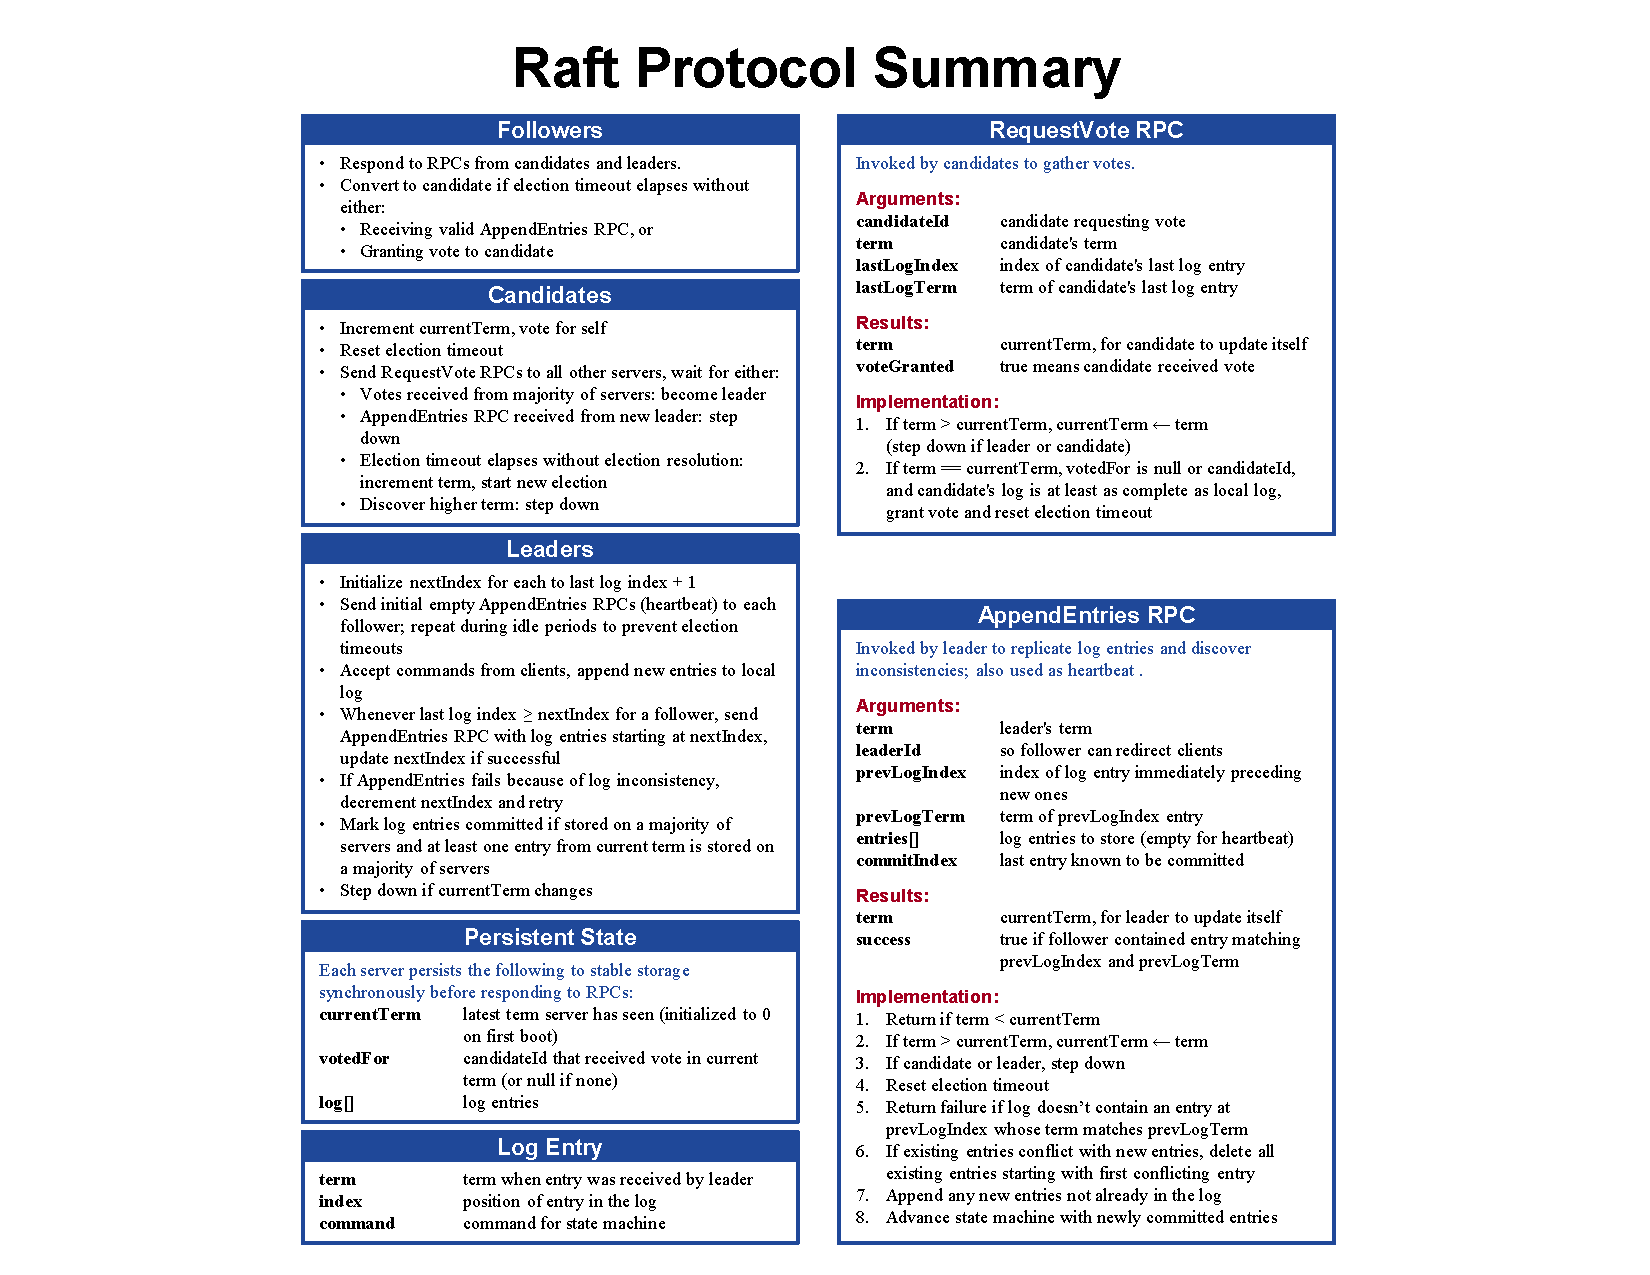
\includegraphics[width=6.0in, trim=2in 0.1in 2in 0.1in,clip=true]{userstudymaterials/raftsummary}
}
\vspace{-3ex}
\vcaption[Raft summary]{
Raft summary used in the user study.
This is an earlier version of Figure~\ref{fig:basicraft:cheatsheet}.
}
\label{fig:appendix:userstudy:raftsummary}
\end{figure}


\begin{figure}
\centering
\fbox{
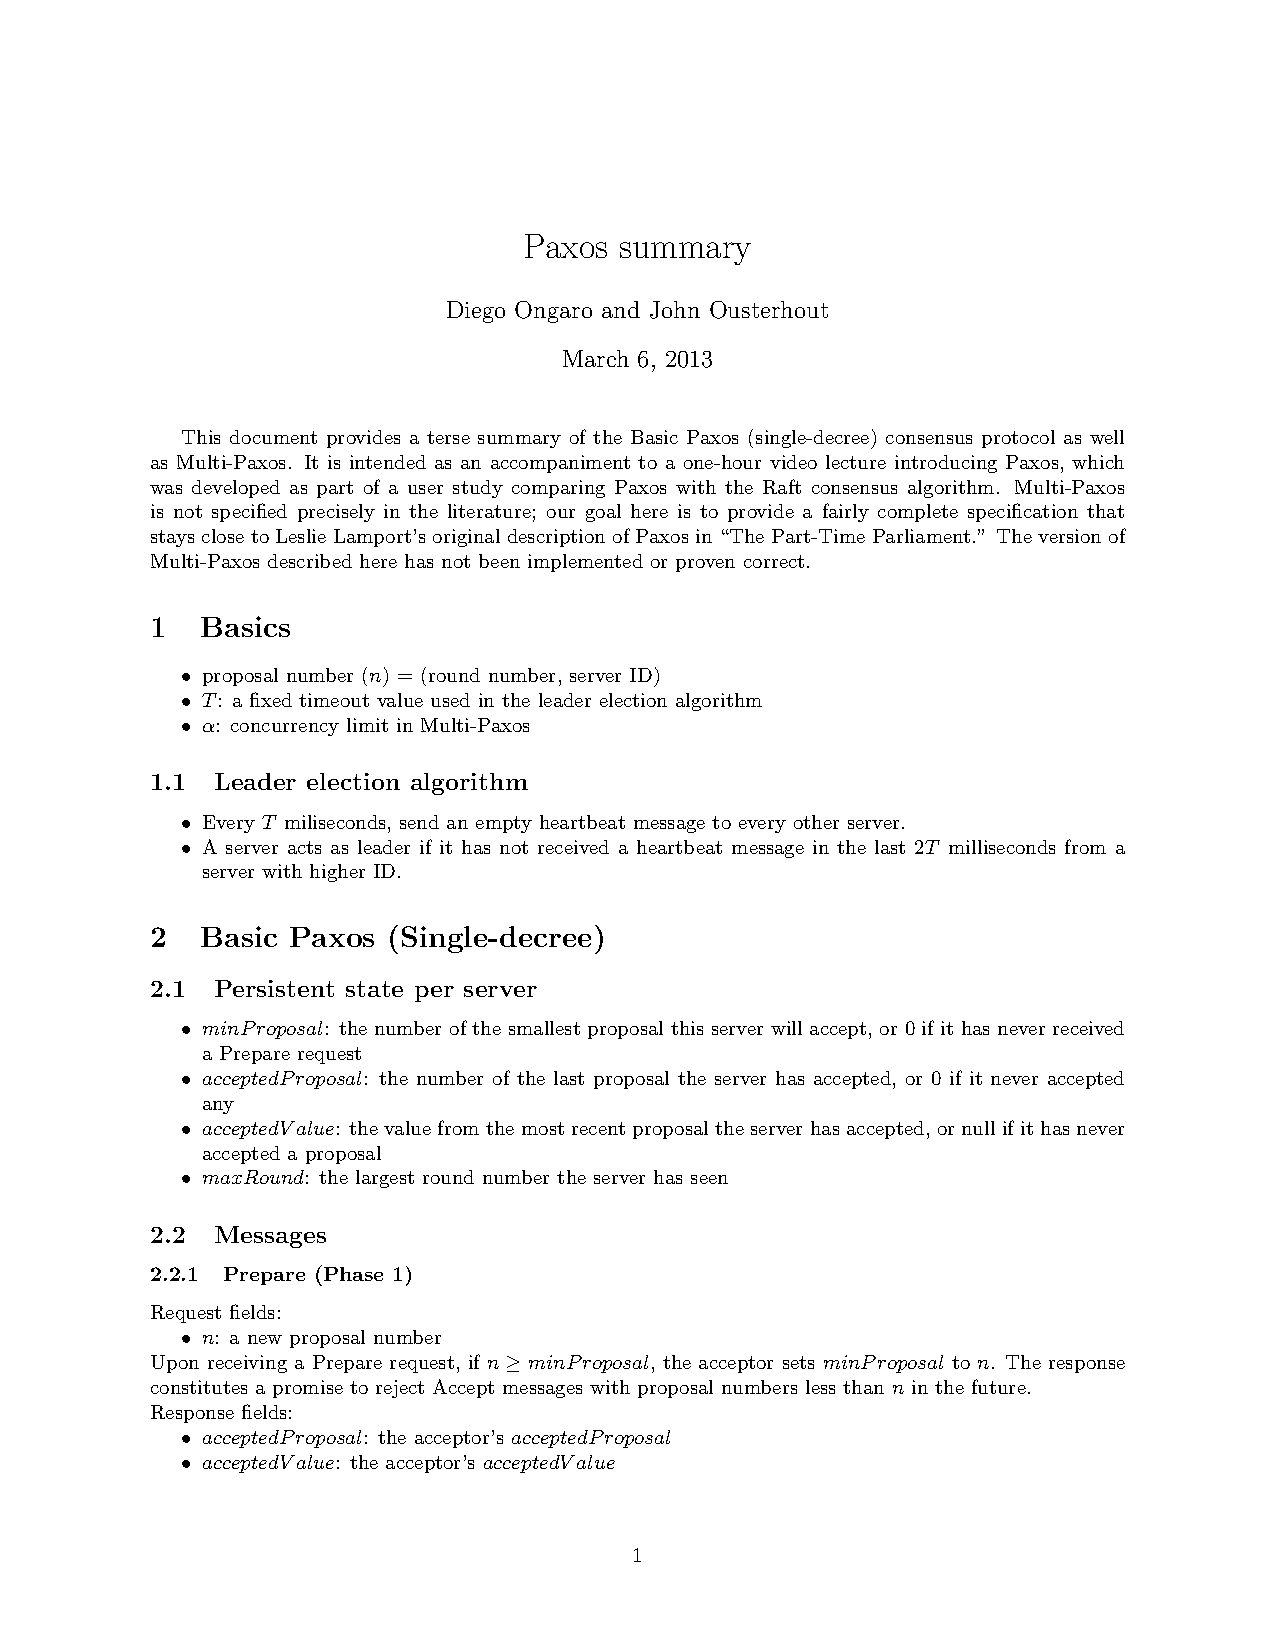
\includegraphics[page=1,width=6.0in,trim=.75in .9in .75in .9in,clip=true]{userstudymaterials/paxossummary}
}
\vspace{-3ex}
\vcaption[Paxos summary, page 1 of 4]{
Paxos summary used in the user study, page 1 of 4.
}
\label{fig:appendix:userstudy:paxossummary1}
\end{figure}

\begin{figure}
\centering
\fbox{
\includegraphics[page=2,width=6.0in,trim=.75in .9in .75in .9in,clip=true]{userstudymaterials/paxossummary}
}
\vspace{-3ex}
\vcaption[Paxos summary, page 2 of 4]{
Paxos summary used in the user study, page 2 of 4.
}
\label{fig:appendix:userstudy:paxossummary2}
\end{figure}

\begin{figure}
\centering
\fbox{
\includegraphics[page=3,width=6.0in,trim=.75in .9in .75in .9in,clip=true]{userstudymaterials/paxossummary}
}
\vspace{-3ex}
\vcaption[Paxos summary, page 3 of 4]{
Paxos summary used in the user study, page 3 of 4.
}
\label{fig:appendix:userstudy:paxossummary3}
\end{figure}

\begin{figure}
\centering
\fbox{
\includegraphics[page=4,width=6.0in,trim=.75in 6.5in .75in .9in,clip=true]{userstudymaterials/paxossummary}
}
\vspace{-3ex}
\vcaption[Paxos summary, page 4 of 4]{
Paxos summary used in the user study, page 4 of 4.
}
\label{fig:appendix:userstudy:paxossummary4}
\end{figure}

\end{enumerate}
